\documentclass[a4paper,10pt]{article}
\usepackage[utf8]{inputenc}
\usepackage{hyperref}
\usepackage{listings}
\usepackage{xcolor}
\lstset { %
    language=C,
    backgroundcolor=\color{black!5}, % set backgroundcolor
    basicstyle=\footnotesize,% basic font setting
}

%opening
\title{Malware}
\author{Guillaume Bonfante}

\usepackage{tikz}

\usetikzlibrary{shapes}
\usetikzlibrary{arrows}
\usetikzlibrary{shadows}
\usetikzlibrary{positioning}

\begin{document}

\maketitle

\section{Introduction}

Securité vs sûreté : \\

La sûreté consiste à vérifier que le système fonctionne correctemenet, tandis que la sécurité introduit le principe d'attaquant, le système fonctionne correctement, mais un attaquant essaye de le détourner.

\paragraph*{}
Cours de 14 séances, les 7 premiers nous allons jouer le rôle des méchants, et les 7 suivants le rôle des gentils.

\paragraph*{}
Les attaques sont fréquentes et ciblent les pays à fort PIB, mais pas seulement. Par exemple, il y a un intérêt à faire du spam, ou des ransomware à des gens choisis dans ces pays. Un autre tye d'attaque moins documenté, sont les attaque étatiques (stuxnet). Un attaque bien connue est WannaCry, car les machines n'étaient pas mise à jour (le responsable informatique souhaitait tout mettre à jour, et le responsable de production a refusé d'arrêter la chaîne poue un ``éventuel problème'', après un calcul de risque ils ont estimé que c'était plus rentable de ne rien arrêter)

\paragraph*{}
Quelques chiffres :
\begin{itemize}
 \item 10 millions : estimation du nombre d'ordinateurs infectés par conficker en 2008 dans plus de 190 pays.
 \item 12 milliards de dollars : coûts estimé des dégâts de Zues en 2010-2012.
 \item 323 000 nouveaux malwares chaque jour en 2016 (selon Kaspersky)
\end{itemize}

\section{Un exemple - Stuxnet}
\begin{center}
  Rapport -- Ralph Langner : ``how to kill a centrifuge''
\end{center}

\paragraph*{}
L'objectif était de ralentir le ncucléaire iranien en attaquant les centrifuges qui enrigissent l'uranium. Quelqu'un s'est introduit sur le site, puis ont localisé tout le matériel, se mettre sur le réseau interne, et enfin attaquer le matériel.

2 scénarios ont été proposé à Obama : un ou on changeait la vitesse des centrifuges pour les faire chauffer et casser, en changeant la valeur des capteurs, ou bien les faire sauter, en augmentant la pression dans certaines gauges.

Pour trouver de l'info sur les virus et des exemples : \url{https://www.botnets.fr/wiki/Main_Page}

\paragraph*{}
Dès qu'une machine lance word, on a tout ce qu'on veut pour faire ce qu'on veut. Word requiert les dll pour dns api, et ncryptssl, ce qui permet de chiffrer une communication entre notre machine et celle-ci.

\section{Un executable}

Un executable est une donnée stockée sur un ordinateur, et se transforme ne executable une fois qu'il est interprêté par un ordinateur.

Un malware est un programme, et de ce fait (théorème, 1940) il ne peut être détecté.

Preuve :
 $P=^?M$ (le programme est un malware, il contient donc exactement les même données que M). Il suffirait donc de vérifier octet par octet qu'ils sont identiques.\\
 En revanche, on a besoin de mieux que ça, on veut que $\left[P\right] =^? \left[M\right]$, c'est à dire que P et M ont les mêmes effets, pas le même code.
\paragraph*{}
 Or, on ne peut pas comparer si deux programmes font exactement la même chose. C'est impossible.

 \section{TP}
 
 On écrit un programme en C pour afficher l'adresse d'une variable qu'on stocke dans la mémoire d'un programme : 
 
\begin{lstlisting}
  #include "stdafx.h"
  
  int _tmain(int argc, _TCHAR* argv[])
 {
    int a = 0x12345678;
    printf("%d\n", & a)
    printf("Hello World");
    while(1);
    return 0;
  }
  
\end{lstlisting}

On va modifier ce snippet pour afficher le contenu en case mémoire et analyser comment sont stockés les ints.

On fait un programme qui va aller lire toutes les cases mémoires le plus loin possible en C (voir VM) : 
\begin{itemize}
 \item La lecture bloque à 0x0041b000.
 \item L'écriture bloque en 0x00405000.
\end{itemize}

La mémoire est découpée en bloc de kilo octets (1000 en hexa).
4 droits, la lecture, l'écriture, executer (il y a des cases executables ou non executables, et finalement le dernier, le droit de l'administrateur (toutes celles qui vont toucher le materiel, interdites pour un utilisateur normal).


Sur windows, tous les executables commencent par MZ, on dit que c'est le header.
\begin{center}
 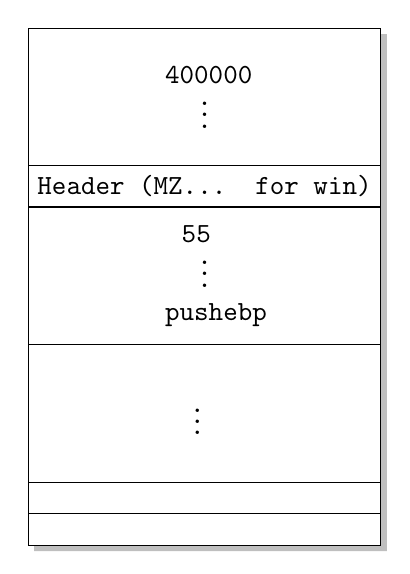
\begin{tikzpicture} [
            % ----- Node definitions ----- %
            dirtablenode/.style = {
                    draw,
                rectangle, 
                rectangle split,
                rectangle split parts = #1,
                fill = white!5,
                align=center,
                drop shadow,
                font=\ttfamily
            },
    ]
    
            % ----- Node constructions ----- %
        \node [dirtablenode=6] (directory) {
            \nodepart{one}
                \parbox[t][15mm][c]{1cm}{400000 \\ \centering \vdots}
            \nodepart[]{two}   
                Header (MZ... for win)
            \nodepart{three} 
		\parbox[t][15mm][c]{1cm}{55\\ \centering \vdots \\ pushebp}
            \nodepart{four} 
                \parbox[t][15mm][c]{1cm}{\vdots}
        };
          
\end{tikzpicture}


\end{center}

Tous les programmes ont donc une structure comme celle ci : 


\begin{center}
 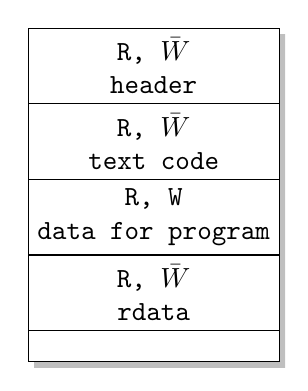
\begin{tikzpicture} [
            % ----- Node definitions ----- %
            dirtablenode/.style = {
                    draw,
                rectangle, 
                rectangle split,
                rectangle split parts = #1,
                fill = white!5,
                align=center,
                drop shadow,
                font=\ttfamily
            },
    ]
    
            % ----- Node constructions ----- %
        \node [dirtablenode=5] (directory) {
            \nodepart[]{one}
                R, $\bar{W}$ \\ header
            \nodepart[]{two}   
		R, $\bar{W}$ \\ text code
            \nodepart[]{three} 
		R, W \\data for program
            \nodepart[]{four} 
		R, $\bar{W}$ \\rdata
        };
          
\end{tikzpicture}
\end{center}

Le Header fait en réalité 1000 Ko, et seuelement 200Ko sont réellement utilisés, on peuut écrire environ n'importe quoi dedans.

\paragraph*{}
On peut lire les octets des fonctions aussi : 

\begin{lstlisting}
#include "stdafx.h"
  
  int _tmain(int argc, _TCHAR* argv[])
 {
    char* q = (char*) printf;
    printf("%x\n", q[0])
    printf("Hello World");
    while(1);
    return 0;
  }
 
\end{lstlisting}

Ce petit programme nous permet de voir que printf commence par 6a. En particulier, on peut aussi afficher la meme chose pour des fonctions donnant des autorisations de modifications de fichier, par exemple virtual mem protect. 

\paragraph*{}
Le ``jeu'' pour un hacker est de cacher les appels fait aux fonctions systèmes pour pas qu'on voit l'execution du programme. 
Pourquoi ? Car sur IDA (voir VM), on peut analyser l'executable et voir les fonctions systèmes auxquels le programme fait appel. Si une image fait appel à l'api dns, c'est pas trop normal par exemple, et toutes ces fonctions sont écrites au début.

\begin{figure}[h!]
 \centering	
 \includegraphics[width=\textwidth]{malware/ida}
 \caption{Disassembly with ida}
\end{figure}

La solution est de se débarasser de printf en cherchant son pointeur d'instruction et en accédant au code de la fonction.

\begin{lstlisting}
#include "stdafx.h"
  
  int _tmain(int argc, _TCHAR* argv[])
 {
    char* p = (char*) scanf;
    char* q = (char*) printf;
    printf("%p %p", p, q)
    while(1);
    return 0;
  }
 
\end{lstlisting}

L'écart entre les deux est de 1200, printf = scanf - 1200.
On enlève alors la ref à printf et on la remplace par scanf - 1200, puis on va bouger le pointeur de fonction pour executer les instructions présente à p.

\begin{lstlisting}
#include "stdafx.h"
//structure de la fonction printf : 
typdef vois (type_function)(const char *, ...); 

  int _tmain(int argc, _TCHAR* argv[])
 {
    char* p = (char*) scanf;
    char* q = p - 1200;
    type_function f;
    f = (type_function) p;
    f("Hello World");
    while(1);
    return 0;
  }
 
\end{lstlisting}

\section{Instructions en assembleur}

\subsection{Les registres}

Les registres de stockage sont :
\begin{itemize}
 \item EAX
 \item EBX
 \item ECX
 \item EDX
\end{itemize}

Ceux pour stocker les chaines de charactères : 
\begin{itemize}
 \item ESI
 \item EDI
\end{itemize}

Ceux pour la pile et les arguments de la fonction en cours : 
\begin{itemize}
 \item ESP (pile)
 \item EBP (arguments)
\end{itemize}

Le pointeur d'instruction : 
\begin{itemize}
 \item EIP (or RIP), on en peut pas faire un mov dessus, c'est interdit.
\end{itemize}

Les registres historiques : 
\begin{itemize}
 \item CS, DS, ES, FS (L'OS utilise ce registre pour stocker des infos), GS, SS
\end{itemize}

Voir ensuite les \href{https://en.wikipedia.org/wiki/Control_register}{Control Registers}	for OS processor.

\paragraph*{}
Il est extremement difficile d'obtenir la liste des instructions x64 processeur, certains projets essayent cependant d'en établir une liste. Les projets open source \href{http://www.capstone-engine.org/}{Capstone} et \href{https://github.com/zyantific/zydis}{Zydis} par exemple.

\subsection{L'assembleur}
\begin{lstlisting}
 mov eax, ebx             ; eax = ebx
 mov eax, 0x1234          ; eax = 0x1234
 mov eax, [ebx]           ; eax = ebx
 mov eax, dword ptr [ebx]
 mov eax, [ebx + 4*ecx]   ; eax = ebx[ecx]
 mov eax, fs:[0x30]          ; eas = fs[30]
\end{lstlisting}
NB : sur cette avant dernière instruction, on peut avoir un 1*, 2*, ou 4*.

\paragraph*{}
\begin{lstlisting}
 mov [eax], ebx
 mov [eax] 0x1234
 mov [eax], [ebx]
\end{lstlisting}

Cette dernière instruction n'est pas de l'assembleur, elle existe en MASM (asm microsoft) mais elle est simplement recompilée en  instructions élémentaires.

Pour mettre à zero un registre :
\begin{lstlisting}
 xor eax, eax
\end{lstlisting}

\paragraph*{}
Pour déplacer le pointeur d'instruction :
\begin{lstlisting}
 jmp 0x4000 000 ; EIP = 0x400 000
 jmp [0x1234]   ; EIP = *(0x1234)
 jmp eax
\end{lstlisting}

Les deux ernières instructions sont des cauchemards pour retracer où le pointeur d'instruction va, et pourtant elles sont présentes dans quasi tous les executables.

Exemple : 
On souhaite appeler printf, qui n'est pas présent dans notre cote (sur windows il est dans une dll) dans l'executable, on a alors stocké quelque part l'adresse de printf dans une case mémoire. tous les appels à printf sont alors compilés par des jumps à cette adresse là.

\paragraph*{}
Il y a toute une liste d'instructions de jump conditionnels (voir slides ou en ligne). 

\subsection{Un appel de fonction}

On appelle ici la fonction dont l'adresse est stockée en 1234 : 
\begin{lstlisting}
 push eax
 push 0x1234
 pop eax  ; dépile et stock le res dans eax
 call [0x1234] ; or call eax
\end{lstlisting}

\section{Code obfuscation}

On veut obfusquer le code suivant : 

\begin{lstlisting}
#include "stdafx.h"
char chaine [] = "Hello world";

  int _tmain(int argc, _TCHAR* argv[])
 {
    printf(chaine)
    while(1);
    return 0;
  }
 
\end{lstlisting}

On utiliise un opérateur idempotent (XOR) pour chiffrer le hello world : 

\begin{lstlisting}
#include "stdafx.h"
char chaine [] = "Hello world";

  int _tmain(int argc, _TCHAR* argv[])
 {
    for (int i=0, i < 12; ++i) {
      print("\\x%02x", chaine[i] ^ 0x42);
    }
    while(1);
    return 0;
  }
 
\end{lstlisting}

Le programme sort alors le résultat suivant : 
\begin{lstlisting}
 \x0a\x27\x2e\x2e\x2d\x62\x35\x2d\x30\x2e\x26\x42
\end{lstlisting}

On modifie alors notre code afin que le hello world soit totalement caché : 

\begin{lstlisting}
#include "stdafx.h"
char chaine [] = "\x0a\x27\x2e\x2e\x2d\x62\x35\x2d\x30\x2e\x26\x42";

  int _tmain(int argc, _TCHAR* argv[])
 {
    for (int i=0, i < 12; ++i) {
	  chaine[i] = chaine[i] ^ 0x42;
	}    
    print(chaine);
    while(1);
    return 0;
  }
 
\end{lstlisting}



\end{document}
